\documentclass[../../thesis.tex]{subfiles}
\graphicspath{{./resources/} }
\begin{document}


\section{Creation of configuration groups}\label{sec:group_sampling:creation_of_groups}

In this section, we tackle the problem of adapting the method described by \citet{saltelli2008global}
to configuration options. We especially try to handle the problem of constraints among the
features during group creation. We devise two strategies to create groups on features and
handle the complexity of constraints during group creation.
In the previous section, we identified several problems the constraints cause when creating
groups of features. Both methods described in the following sections aim to mitigate these obstacles
in order to still create groups in the presence of constraints.


\subsection{Maximizing Hamming distance}\label{sec:group_sampling:creation_of_groups:hamming}

This method aims to generate groupings of features without any previous analysis of the feature model.
The main idea is to create groups of features with minimal overlap between them.
In the best-case scenario of a feature model with only independent features,
this would create groups without any overlap between them and thus completely distinct
sets of features.
To measure the overlap between two groups of features we use the Hamming distance between the two groups.
\begin{equation} \label{eq:group_sampling:creation_of_groups:hamming:hamming_distance}
    \begin{aligned}
        D_{H} = \sum_{i=1}^{n} f(A_i, B_i)
        \\ \\
        f(A,B) =
        \left\{
        \begin{array}{ll}
            0 & \mbox{if } A = B \\
            1 & \mbox{else }
        \end{array}
        \right.
    \end{aligned}
\end{equation}
This means, the Hamming distance between two groups is equal to the amount
of features which are not in both groups.

Since we do not have a hard constraint of no overlap between groups, mandatory features
are allowed to be in all groups. This allows us to ignore them during group creation due to the fact,
that their influence on performance does not contribute to performance variation.
The complexity of mutually exclusive groups and features with implications
is implicitly solved by the SAT-Solver, since it is responsible to create valid configurations.

We also need to define how many features should be contained in a group.
Otherwise, we leave it open to the SAT-Solver to determine the number of features in a group, which
would result in very uneven group sizes due to the nature of SAT-Solvers.
Since we do not have any previous knowledge of the number of independent features, mutually exclusive
groups or features with implications, the most straightforward answer to the number of features which
should be contained in a group would be:

\begin{equation} \label{eq:group_sampling:creation_of_groups:hamming:no_of_features}
    Features\ in \ group=\myfloor{\frac{No.\ Features}{Group\ size}}
\end{equation}



\subsection{Grouping independent features}\label{sec:group_sampling:creation_of_groups:mutex}

While grouping features using the Hamming distance between the groups simplifies the process
of creating groups by pushing the complexity to the SAT-Solver. This method provides a more
hands-on approach. We analyze the feature model and determine the independent features
and the groups of mutually exclusive features. With the knowledge we have, we can more easily
create valid groups of features.


\subsubsection{Groups with mutually exclusive features}

To create groups among mutually exclusive features, we want to pick one feature out of each group of
mutually exclusive features, if possible. With this, we get the maximal amount of features we can group
together across all mutually exclusive groups. If we assume, we have a feature model with two alternative groups, the maximal amount of
features, we can group together is two, since only one feature out of each alternative group can be selected.
To look for mutually exclusive features in a feature model, we can use the SAT-Solver.
By enabling each combination of any two features and checking, if there is a valid configuration, we can find out which
two features are mutually exclusive. The pairs of mutually exclusive features help us to determine
the mutually exclusive groups. In a mutually exclusive group, only one feature of the group can be enabled.
This means all features in the group are mutually exclusive with all other features in the group.
If we translate the mutually exclusive relationship between features into an undirected graph,
where the nodes represent the features and the edges the mutually exclusive relationship,
we can reformulate the problem of finding the groups as the clique problem \cite{bron1973algorithm}.
The cliques in the graph represent a mutually exclusive group because all nodes in the clique are fully connected.
\autoref{fig:group_sampling:mutex_graph} depicts such a graph.


\begin{figure}[htp]
    \begin{center}
        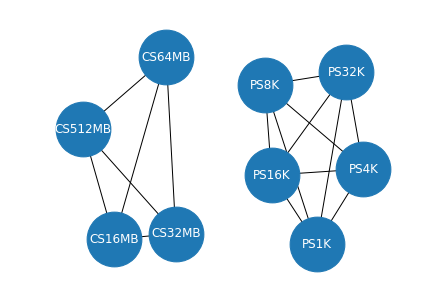
\includegraphics[width=0.49\textwidth]{graphs/mutex_graph.png}
    \end{center}

    \caption[Graph of mutually exclusive features - BerkeleyDB]{
        Graph of mutually exclusive features in the BerkeleyDB dataset.
    }\label{fig:group_sampling:mutex_graph}
\end{figure}



\begin{figure}[htp]
    \begin{center}
        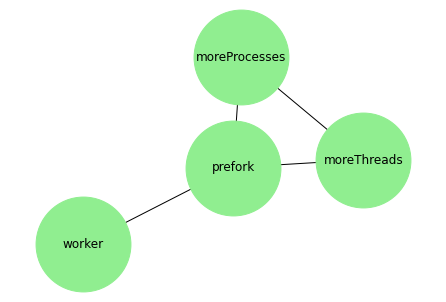
\includegraphics[width=0.49\textwidth]{graphs/mutex_apache_part.png}
    \end{center}
    \caption[Graph of mutually exclusive features - Apache]{
        Partial graph of mutually exclusive features in the Apache dataset.
    }\label{fig:group_sampling:mutex_graph_part}
\end{figure}

When we select features out of mutually exclusive groups we have to be aware, that mutually exclusive groups
can overlap. This presents a problem when we select an overlapping feature. To illustrate the problem,
a subgraph from the mutually exclusive relationships in the Apache dataset is presented in \autoref{fig:group_sampling:mutex_graph_part}.
The mutually exclusive groups, the cliques, in this example would be
\textit{worker, prefork} and \textit{prefork, moreProcesses, moreThreads}. Since \textit{prefork} is contained
in both groups, if we pick this feature, we can not pick any feature of the other mutually exclusive group.
To circumvent this problem, instead of choosing one feature out of each mutually exclusive group,
we choose one feature out of each component\footnote{A component of an undirected graph is connected subgraph has no edges to any other graph}.
This leaves us with smaller groups since fewer features can be selected for each group,
but a more equal distribution of selected features
in connected mutually exclusive groups.


\subsubsection{Groups with independent features}
The independent features are all features, which can be disabled and are not in any of the mutually exclusive groups.
Not all features in a feature model which are modelled as optional are really optional.
\Citet{benavides2010automated} describe these features, features which are included in all configurations, despite being modelled
as optional, as false optional features.
So to determine the independent features we need to determine features, which really can be enabled optionally.
This can be done by iterating overall features and checking if a valid configuration exists where the feature is disabled
\cite{schroter2013automated}. 
The set of features which can be disabled without the features contained in a group of mutually exclusive features is
the set of independent features. Since the independent features are not bound by any constraints, we can randomly
assign a feature to a group without being concerned about violating any constraints.

\subsubsection{}
We can now combine both approaches for grouping mutually exclusive features and independent features
to create groups over the whole feature model. We are still limited by the fact, that we can not create
more distinct groups than the amount of the smallest mutually exclusive component. This would mean, that
we can't cover all features in one round of grouping. We can circumvent this problem by simply allowing for
mutually exclusive features to be in multiple groups. This lets us create more groups, but makes it harder
to determine the influence of a feature that is assigned to multiple groups.

To actually generate a group, we need to define how many features are in a group.
The amount of features from the mutually exclusive features is simply the amount
of components $|C|$ in the mutually exclusive graph.
The amount of features in a group can be described with the following formula:

\begin{equation} \label{eq:group_sampling:creation_of_groups:hamming:mutex}
    N=\myfloor{\frac{No.\ independent\ features}{Group\ size}}
\end{equation}



\begin{equation} \label{eq:group_sampling:creation_of_groups:hamming:mutex}
    Features\ in\ group = N + |C| + mandatory\ features
\end{equation}



\subsubsection{}
We can see samples created from both variations in \autoref{fig:group_sampling:samples}.
Each row represents a configuration and each column represents a feature. A feature is selected,
if the block is black, otherwise it is not selected. A round of groupings is separated by
a horizontal line.
Looking at the figure, we can already identify a problem both varients have.
The differences between the rounds of groupings are minimal, caused by the use of an SAT-Solver.
We tackle this problem in \autoref{sec:optimization:feature_coverage}


\begin{figure}[htp]
    \begin{center}

        % 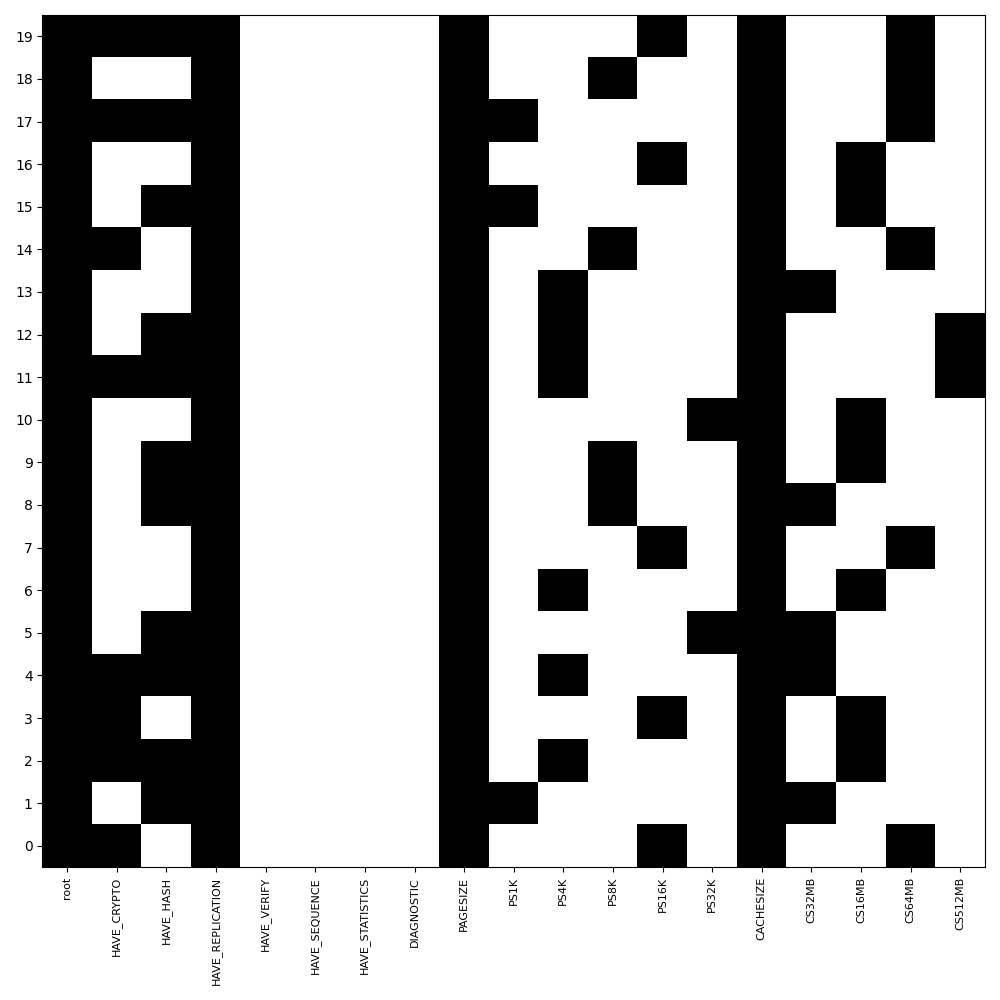
\includegraphics[width=0.49\textwidth]{sampling_distribution/rs_diversity_promotion_ss20.png}
        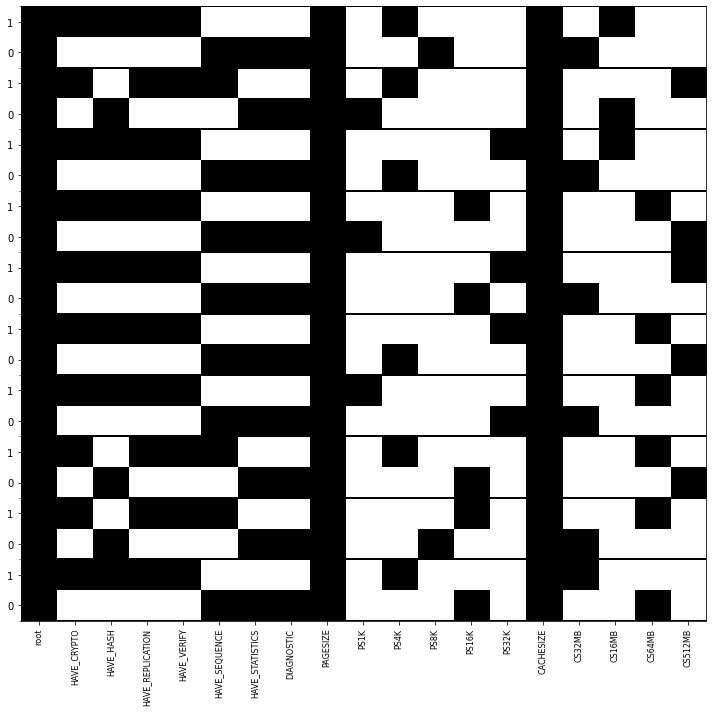
\includegraphics[width=0.49\textwidth]{sampling_distribution/gs_hemming_ss20_gs5.png}
        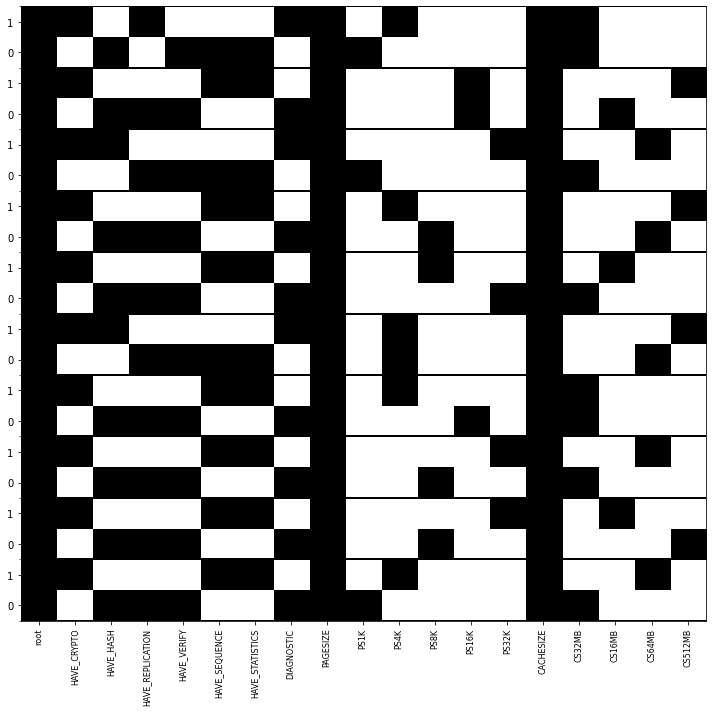
\includegraphics[width=0.49\textwidth]{sampling_distribution/gs_mutex_ss20_gs5.png}
    \end{center}

    \caption[Group Sampling - Samples]{
        Samples generated on the BerkeleyDB Dataset by both variations to generate groups.
        \textbf{Left:}  Group Sampling - Hemming Distance - Group Size 2 - Groupings 10
        \textbf{Right:} Group Sampling - Independent features - Group Size 2 - Groupings 10
    }\label{fig:group_sampling:samples}
\end{figure}


\end{document}


